\documentclass[12pt]{report}
\usepackage[utf8]{inputenc}
\usepackage[russian]{babel}
%\usepackage[14pt]{extsizes}
\usepackage{listings}
\usepackage{graphicx}
\usepackage{amsmath,amsfonts,amssymb,amsthm,mathtools} 
\usepackage{pgfplots}
\usepackage{filecontents}
\usepackage{indentfirst}
\usepackage{eucal}
\usepackage{amsmath}
\usepackage{enumitem}
\frenchspacing

\usepackage{indentfirst} % Красная строка


%\usetikzlibrary{datavisualization}
%\usetikzlibrary{datavisualization.formats.functions}

\usepackage{amsmath}




% Для листинга кода:
\lstset{ %
language=haskell,                 % выбор языка для подсветки (здесь это С)
basicstyle=\small\sffamily, % размер и начертание шрифта для подсветки кода
numbers=left,               % где поставить нумерацию строк (слева\справа)
numberstyle=\tiny,           % размер шрифта для номеров строк
stepnumber=1,                   % размер шага между двумя номерами строк
numbersep=5pt,                % как далеко отстоят номера строк от подсвечиваемого кода
showspaces=false,            % показывать или нет пробелы специальными отступами
showstringspaces=false,      % показывать или нет пробелы в строках
showtabs=false,             % показывать или нет табуляцию в строках
frame=single,              % рисовать рамку вокруг кода
tabsize=2,                 % размер табуляции по умолчанию равен 2 пробелам
captionpos=t,              % позиция заголовка вверху [t] или внизу [b] 
breaklines=true,           % автоматически переносить строки (да\нет)
breakatwhitespace=false, % переносить строки только если есть пробел
escapeinside={\#*}{*)}   % если нужно добавить комментарии в коде
}

\usepackage[left=2cm,right=2cm, top=2cm,bottom=2cm,bindingoffset=0cm]{geometry}
% Для измененных титулов глав:
\usepackage{titlesec, blindtext, color} % подключаем нужные пакеты
\definecolor{gray75}{gray}{0.75} % определяем цвет
\newcommand{\hsp}{\hspace{20pt}} % длина линии в 20pt
% titleformat определяет стиль
\titleformat{\chapter}[hang]{\Huge\bfseries}{\thechapter\hsp\textcolor{gray75}{|}\hsp}{0pt}{\Huge\bfseries}


% plot
\usepackage{pgfplots}
\usepackage{filecontents}
\usetikzlibrary{datavisualization}
\usetikzlibrary{datavisualization.formats.functions}
\RequirePackage[
  style=gost-numeric,
  language=auto,
  autolang=other,
  sorting=none,
]{biblatex}

\addbibresource{bib.bib}
\begin{document}
%\def\chaptername{} % убирает "Глава"
\thispagestyle{empty}
\begin{titlepage}
	\noindent \begin{minipage}{0.15\textwidth}
	
\includegraphics[width=\linewidth]{b_logo}
	\end{minipage}
	\noindent\begin{minipage}{0.9\textwidth}\centering
		\textbf{Министерство науки и высшего образования Российской Федерации}\\
		\textbf{Федеральное государственное бюджетное образовательное учреждение высшего образования}\\
		\textbf{~~~«Московский государственный технический университет имени Н.Э.~Баумана}\\
		\textbf{(национальный исследовательский университет)»}\\
		\textbf{(МГТУ им. Н.Э.~Баумана)}
	\end{minipage}
	
	\noindent\rule{18cm}{3pt}
	\newline\newline
	\noindent ФАКУЛЬТЕТ $\underline{\text{«Информатика и системы управления»}}$ \newline\newline
	\noindent КАФЕДРА $\underline{\text{«Программное обеспечение ЭВМ и информационные технологии»}}$\newline\newline\newline\newline\newline
	
	
	\begin{center}
		\noindent\begin{minipage}{1.3\textwidth}\centering
			\Large\textbf{  Отчёт по лабораторной работе №4 по дисциплине}\newline
			\textbf{ "Методы машинного обучения"}\newline\newline
		\end{minipage}
	\end{center}
	
	\noindent\textbf{Тема} $\underline{\text{Наивный байесовский классификатор для фильтрации спама}}$\newline\newline
	\noindent\textbf{Студент} $\underline{\text{Варламова Е. А.}}$\newline\newline
	\noindent\textbf{Группа} $\underline{\text{ИУ7-23М}}$\newline\newline
	\noindent\textbf{Оценка (баллы)} $\underline{\text{~~~~~~~~~~~~~~~~~~~~~~~~~~~}}$\newline\newline
	\noindent\textbf{Преподаватели} $\underline{\text{Солодовников Владимир Игоревич}}$\newline\newline\newline
	
	\begin{center}
		\vfill
		Москва~---~\the\year
		~г.
	\end{center}
\end{titlepage}
\large
\setcounter{page}{2}
\def\contentsname{СОДЕРЖАНИЕ}
\renewcommand{\contentsname}{СОДЕРЖАНИЕ}
\tableofcontents
\renewcommand\labelitemi{---}
\newpage
\chapter{Теоретическая часть}

Фильтрация спама является необходимой для обеспечения безопасности и эффективности работы в сети. Спам может содержать вредоносные ссылки, вирусы или фишинговые атаки, которые могут нанести ущерб вашим данным или устройствам. Кроме того, спам может засорять почтовый ящик или другие коммуникационные каналы, делая их менее эффективными для передачи важных сообщений. Фильтрация спама помогает защитить вас от нежелательного контента и обеспечивает более продуктивное использование интернета и электронной почты.

Целью данной лабораторной работы является применение наивного байесовского классификатора для фильтрации спама.
Для этого необходимо решить следующие задачи:
\begin{itemize}
    \item формализовать задачу;
    \item описать алгоритм наивного байесовского классификатора;
    \item привести схему ПО, реализующего фильтрацию спама с помощью наивного байесовского классификатора;
    \item привести особенности реализации ПО, решающего поставленную задачу;
    \item провести исследование зависимости результатов точности классификации в зависимости от алгоритма векторизации, применяемого до классификации.
\end{itemize}

\section{Постановка задачи}

Решить задачу фильтрации спама с использованием наивного байесовского классификатора, основанного на принципе максимума апостериорной вероятности. В качестве исходных данных можно использовать данные с сайта Kaggle (SMS Spam Collection Dataset) (можно какой-то другой датасет).
В выполнения работы:
\begin{enumerate}
    \item Осуществить предобработку данных. Сформировать обучающий и тестовый наборы данных.
    \item Построить наивный байесовский классификатор.
    \item Оценить качество работы классификатора. 
\end{enumerate}

\section{Алгоритм наивного байесовского классификатора}
Классификация с использованием наивного байесовского классификатора основана на применении теоремы Байеса. Пусть дан набор объектов $X = (x_1, x_2, ..., x_n)$ и метки классов $Y = (y_1, y_2, ..., y_m)$. Наивный байесовский классификатор предполагает, что все признаки объектов независимы друг от друга при условии класса. Таким образом, вероятность принадлежности объекта x к классу y может быть вычислена по формуле:

\begin{equation}
  P(y|x) = P(x|y)P(y)/P(x)  
\end{equation}
    
где 
\begin{enumerate}
    \item $P(y|x)$ - вероятность принадлежности объекта $x$ к классу $y$;
    \item $P(x|y)$ - вероятность объекта $x$ при условии класса $y$;
    \item $P(y)$ - априорная вероятность класса $y$;
    \item $P(x) $- вероятность объекта $x$.
\end{enumerate}

Для наивного байесовского классификатора используются различные модели для оценки вероятностей $P(x|y)$ и $P(y)$. Например, для категориальных данных можно использовать модель мультиномиального распределения, а для непрерывных данных - модель нормального распределения.

На практике для классификации объекта выбирается класс с наибольшей вероятностью $P(y|x)$:

\begin{equation}
    y' = max_y \in Y P(y|x)
\end{equation}

где $y'$ - предсказанная метка класса для объекта $x$.

Таким образом, наивный байесовский классификатор является простым и эффективным методом классификации, основанным на принципах вероятностного вывода.

\section{Алгоритм векторизации CountVectorizer}
CountVectorizer -- это метод векторизации текстовых данных, который преобразует текстовые данные в матрицу частот слов. Алгоритм работы CountVectorizer можно описать следующим образом:
\begin{enumerate}
    \item Токенизация: Исходный текст разбивается на отдельные слова или токены. Токенизация может проводиться с использованием различных методов, например, разделение по пробелам или использование регулярных выражений.

    \item Построение словаря: CountVectorizer строит словарь всех уникальных слов (токенов) в исходном тексте. Каждому уникальному слову присваивается уникальный индекс.

    \item Подсчет частот слов: Для каждого текста подсчитывается количество вхождений каждого слова из словаря. Эти частоты слов образуют строки матрицы частот слов.

    \item Преобразование векторов: Каждый текст представляется в виде вектора, где каждый элемент соответствует количеству вхождений соответствующего слова из словаря.

    \item Преобразование редких матриц: Поскольку большинство слов в тексте редко встречаются, матрица частот слов будет разреженной. CountVectorizer может сохранять разреженные матрицы для экономии памяти.
\end{enumerate}

\section{Алгоритм векторизации TfidfVectorizer}
TfidfVectorizer - это метод векторизации текстовых данных, который преобразует текстовые данные в матрицу TF-IDF (Term Frequency-Inverse Document Frequency). Алгоритм работы TfidfVectorizer можно описать следующим образом:
\begin{enumerate}
    \item Токенизация: Исходный текст разбивается на отдельные слова или токены. Токенизация может проводиться с использованием различных методов, например, разделение по пробелам или использование регулярных выражений.

    \item  Подсчет TF (Term Frequency): Для каждого текста подсчитывается количество вхождений каждого слова из словаря. Это называется частотой слова в документе (TF). TF показывает, насколько часто слово встречается в данном документе.

    \item Подсчет IDF (Inverse Document Frequency): IDF вычисляется как логарифм отношения общего числа документов к числу документов, содержащих данное слово. IDF показывает, насколько информативно слово является для всех документов.

    \item Вычисление TF-IDF: TF-IDF для каждого слова в документе вычисляется как произведение TF и IDF для этого слова. Это дает вес словам, учитывая как их частоту в текущем документе, так и их уникальность во всей коллекции документов.

    \item Преобразование векторов: Каждый текст представляется в виде вектора, где каждый элемент соответствует значению TF-IDF для соответствующего слова из словаря.

    \item Нормализация векторов: Векторы могут быть нормализованы для улучшения работы моделей машинного обучения.
\end{enumerate}
TfidfVectorizer помогает учитывать не только частоту слова в документе, но и его важность для всей коллекции текстов. Этот метод широко используется в задачах анализа текста, кластеризации и рекомендательных системах.


\section{Схема работы ПО}
На рисунке \ref{fig:scheme} представлена схема работы ПО.
\begin{figure}[h!]
  \centering
  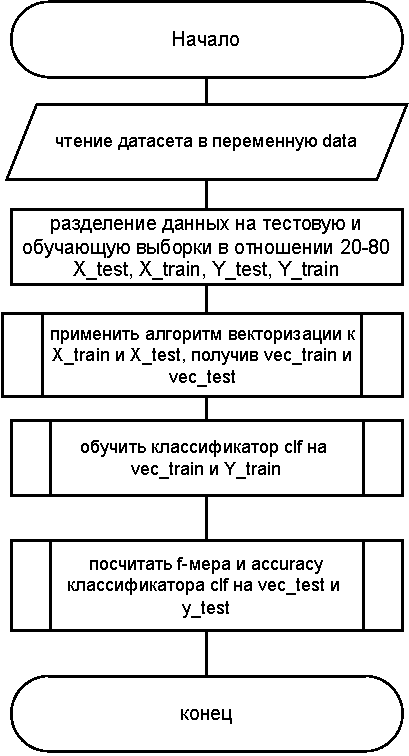
\includegraphics[scale = 0.5]{scheme.pdf}
  \caption{схема работы ПО}
  \label{fig:scheme}
\end{figure}
\chapter{Практическая часть}

\section{Выбор средств разработки}
В качестве языка программирования был использован язык Python, поскольку этот язык кроссплатформенный и для него разработано огромное количество библиотек и модулей, решающих разнообразные задачи. 

В частности, имеются библиотеки, включающие в себя алгоритм наивного байесовского классификатора, а также алгоритмы векторизации текстов  в библиотеке \cite{bib:scipy}.

\section{Исследование ПО}

В листинге \ref{lst:gen1} представлен код, решающий задачу классификации спама.

\begin{lstlisting}[label=lst:gen1,caption=Код классификации спама]
import pandas as pd
from sklearn.feature_extraction.text import CountVectorizer
from sklearn.model_selection import train_test_split
from sklearn.naive_bayes import MultinomialNB
from sklearn.metrics import confusion_matrix, precision_recall_fscore_support, accuracy_score
from nltk.tokenize import word_tokenize
from nltk.corpus import stopwords
from sklearn.feature_extraction.text import TfidfVectorizer
from pymorphy2 import MorphAnalyzer
import warnings

warnings.filterwarnings("ignore")
morph = MorphAnalyzer()
stop_words = set(stopwords.words('english'))
lemma = True

def preprocess_text(text):
    tokens = word_tokenize(text.lower())
    if lemma:
        tokens = [morph.parse(token)[0].normal_form for token in tokens]
    return ' '.join(tokens)

def CountVectorization(X_train, X_test):
    vectorizer = CountVectorizer()
    X_train_counts = vectorizer.fit_transform(X_train)
    X_test_counts = vectorizer.transform(X_test)
    return X_train_counts, X_test_counts
def tfidfVectorization(X_train, X_test):
    tfidf_vectorizer = TfidfVectorizer()
    X_train_counts = tfidf_vectorizer.fit_transform(X_train.apply(preprocess_text))
    X_test_counts = tfidf_vectorizer.transform(X_test.apply(preprocess_text))
    return X_train_counts, X_test_counts

data = pd.read_csv('spam.csv', encoding='latin-1')
data = data[['v1', 'v2']]
data.columns = ['label', 'text']

data['label'] = data['label'].map({'ham': 0, 'spam': 1})
X = data['text']
y = data['label']

X_train, X_test, y_train, y_test = train_test_split(X, y, test_size=0.2, random_state=42)
vecs = ["CountVectorization", "tfidfVectorization"]
i = 0
for vectorization in [CountVectorization, tfidfVectorization]:
    print(vecs[i])
    X_train_counts, X_test_counts = vectorization(X_train, X_test)

    clf = MultinomialNB()
    clf.fit(X_train_counts, y_train)
    
    y_pred = clf.predict(X_test_counts)
    accuracy = accuracy_score(y_test, y_pred)
    precision, recall, f1, _ = precision_recall_fscore_support(y_test, y_pred, average='weighted')
    print("Accuracy: ", accuracy)
    print("f-мера:", f1)
    cm = confusion_matrix(y_test, y_pred)
    print(f"Матрица ошибок:")
    print(cm)
    print()
    i += 1
\end{lstlisting}

\newpage
С помощью разработанного ПО было проведено исследование зависимости точности классификации от алгоритма предобработки текстов (алгоритма векторизации текстов).

\begin{table}[!h]
	\begin{center}
		\caption{\label{tbl1}Результаты работы ПО} 
		\footnotesize
		\begin{tabular}{|l|l|l|l|}
			\hline	
   \multicolumn{1}{|c|}{\begin{tabular}[c]{@{}c@{}}Алгоритм \\ векторизации\end{tabular}} & 
    \multicolumn{1}{c|}{\begin{tabular}[c]{@{}c@{}} Точность (accuracy)\end{tabular}} & 
    \multicolumn{1}{c|}{\begin{tabular}[c]{@{}c@{}}Точность (f-мера)\end{tabular}} & 
   \multicolumn{1}{c|}{\begin{tabular}[c]{@{}c@{}}Матрица ошибок\end{tabular}} \\
\hline CountVectorization & 0.98386 & 0.98352 & [[963   2] [ 16 134]]  \\
\hline tfidfVectorization & 0.96233 & 0.95967 & [[965   0] [ 42 108]] \\
\hline
	\end{tabular}
	\end{center}
\end{table}

Видим, что более простой алгоритм векторизации в паре с наивным байесовским классификатором показал лучший результат классификации.

\printbibliography[title={СПИСОК ИСПОЛЬЗОВАННЫХ\\ ИСТОЧНИКОВ}]
\addcontentsline{toc}{chapter}{СПИСОК ИСПОЛЬЗОВАННЫХ ИСТОЧНИКОВ}

\end{document}